%AMRITA UNIVERSITY PH.D latex template...Created by Chungath, CYS-CBE%

\documentclass[a4paper, 12pt]{report}
%\renewcommand{\bibname}{References}
\usepackage[margin=0.8in]{geometry}
\usepackage{algorithm}
\usepackage{algpseudocode}

\usepackage{bold-extra}
\usepackage{amsmath}
\usepackage{amsfonts}
\usepackage{amssymb}
\usepackage{graphicx}
\usepackage [english]{babel}
\usepackage [autostyle, english = american]{csquotes}
\MakeOuterQuote{"}
%\usepackage[a4paper,top=30mm,bottom=30mm]{geometry}
\usepackage{setspace}
\onehalfspacing
\graphicspath{{images/}}
\usepackage{amsthm}
%\usepackage{hyperref}
%\hypersetup{colourlinks=true,linkcolour=blue}
\usepackage{array}
%\usepackage{parskip}
\usepackage{cite}
\usepackage{longtable}
\usepackage{fancyhdr}
\usepackage{titletoc}
\usepackage{booktabs}
\usepackage{tikz}
\usetikzlibrary{positioning,arrows.meta,fit}
\usepackage{caption}
\usepackage{subcaption}
\usepackage{url}
\theoremstyle{definition}
\newtheorem{Definition}{Definition}[section]

%-------------------------------------------------------------
% title page
\begin{document}
	\pagenumbering{gobble}
	\thispagestyle{empty}
	\begin{large}
		\begin{center}
			{\Large\bfseries{Does Fine-Tuning Beat Prompting? A Controlled, Uncertainty-Aware Comparison of Classical, Zero-Shot and LoRA-Tuned Vision-Language Models for Stance and Target Classification of Malayalam Political Memes}}\\
			\vspace{1.3cm}
			A PROJECT REPORT \\
			\vspace{.1cm}
			Submitted in partial fulfillment for the Degree of\\
			\vspace{.1cm}
			Bachelor of Technology under the\\
			\vspace{.1cm}
			School of Computing\\
			\vspace{1cm}
			
			\normalsize Submitted by \\
\begin{table}[h]
\centering
\begin{tabular}{lr}\hline \\
Register No & Names of Students \\ \\ \hline
\\
AM.SC.U4AIE23007 & Adithya Rajesh \\
AM.SC.U4AIE23026 & Balu M Krishna \\ 
AM.SC.U4AIE23065 & Adithyan \\ \\ \hline 
\end{tabular}
\end{table}



\vfill
			
\includegraphics[scale=0.7]{univA.png}\\
			DEPARTMENT OF COMPUTER SCIENCE AND ENGINEERING\\
			\Large{\textbf{AMRITA VISHWA VIDYAPEETHAM}}\\
			{\large Amritapuri Campus (INDIA)}\\
			\vspace*{.3cm}
			October 2026
		\end{center}
	\end{large}
	%------------------------------------------------------------------------------------
	% bonafide certificate
	\newpage
	\begin{center}
		
		{\large Department of Computer Science and Engineering}\\
		\Large{ \textbf{AMRITA VISHWA VIDYAPEETHAM}}\\
			{\large AMRITAPURI CAMPUS}\\
		\vspace*{2.2cm}
		%\includegraphics[width=5cm,height=5cm,keepaspectratio]{university.jpg}
		\includegraphics[scale=0.5]{univa.png}\\
		\vspace*{1.5cm}
		{\Large \textbf{BONAFIDE CERTIFICATE}}
	\end{center}
	\vspace*{.8cm}
	This is to certify that this is a bonafide record of the project presented by the students whose names are given below during Project Phase I (22AIE498) in partial fulfilment of the requirements of the degree of Bachelor of Technology in Computer Science and Engineering (Artificial Intelligence).\\[1.0cm]

\begin{table}[h]
\centering
\begin{tabular}{lr}
Roll No & Names of Students \\ \\ \hline
\\
AM.SC.U4AIE23007 & Adithya Rajesh \\ 
AM.SC.U4AIE23026 & Balu M Krishna \\
AM.SC.U4AIE23065 & Adithyan \\

\end{tabular}
\end{table}



% Bottom of the page
\begin{flushleft}
  Dr. Veena G\\
(Project Guide)\\  [1cm]

 \texttt{<}Coordinator name here\texttt{>}\\
(Project Coordinator)\\
Designation\\
\end{flushleft}
\begin{flushright}
\texttt{<}Reviewer's Name\texttt{>}\\
(Reviewer)\\
Designation
\end{flushright}




\newpage
	%-----------------------------------------------------------------------------
	\clearpage
	\pagenumbering{roman}
	\tableofcontents
	
	\chapter*{Acknowledgements}
	\addcontentsline{toc}{chapter}{Acknowledgements}	
	We express our sincere gratitude to our project guide, Dr. Veena G, for her guidance, regular feedback and encouragement throughout Project Phase I. We thank the Department of Computer Science and Engineering, Amrita Vishwa Vidyapeetham, Amritapuri Campus, for providing the opportunity and the environment to carry out this work, and the organisers of the DravidianLangTech shared task for the Malayalam meme dataset on which this study is based.\\
	\vspace{1cm}
	\begin{flushright}
		ADITHYA RAJESH\\
		BALU M KRISHNA\\
		ADITHYAN
	\end{flushright}
	\listoffigures
	\addcontentsline{toc}{chapter}{List of figures}
	\listoftables
	\addcontentsline{toc}{chapter}{List of tables}
	\newpage
%\chapter*{Abbreviations}

\chapter*{Abstract}
\addcontentsline{toc}{chapter}{Abstract}
Internet memes are a major vehicle for political opinion in India, yet almost all multimodal meme research targets English and asks whether a meme is hateful, not what stance it takes toward whom. We study a two-level stance task on Malayalam political memes: Level~1 (troll vs.\ support) and Level~2 (target: person, party or both). Using one frozen 500/100 train/test split and one metric (macro-F1 with bootstrap confidence intervals), we compare three families on equal terms: a classical baseline (frozen Swin-Tiny and MuRIL with a residual fusion head), prompt-only inference with a vision-language model (Qwen3-VL-2B, zero-shot and chain-of-thought), and parameter-efficient LoRA fine-tuning of the same Qwen3-VL-2B across rank, seed and minority-oversampling settings. Using the same backbone for prompting and fine-tuning isolates the effect of training from the effect of model choice. We also test whether Grad-CAM heatmaps on the classical baseline are faithful, using deletion and insertion curves against a random-order control.

The main finding is a cautionary one. On a 100-image test set with only four ``support'' memes, no system is significantly better than the classical baseline at Level~1, and the same LoRA configuration varies from 0.38 to 0.51 average macro-F1 across seeds, which is as large as the gaps between methods. Level-2 macro-F1 is 0.394 for the classical baseline, 0.499 for zero-shot prompting and 0.482 $\pm$ 0.026 for LoRA with minority oversampling (three seeds), against 0.349 $\pm$ 0.061 for plain LoRA; plain LoRA frequently collapses to the majority class. Grad-CAM beats random patch ordering on both deletion and insertion for 82--93\% of images ($p<10^{-11}$), so the maps are faithful to the model at their coarse $7\times7$ resolution. We also flag which comparisons to the published reference system we could not verify. Natural-language rationales, cross-lingual transfer and a 7B-scale study are left to Phase~II.\\
\textbf{Keywords:} multimodal meme analysis, Malayalam, vision-language models, LoRA, explainability, Grad-CAM, low-resource languages.\\

\clearpage
\pagenumbering{arabic}
\setcounter{page}{1}
\chapter{Introduction}
\section{Background}

Memes combine an image with a short piece of text and are now one of the main ways people voice political opinion online. In India they are usually written in a regional language, often code-mixed or in a transliterated script, and they depend on local political context that a reader must already know. Automatic analysis of memes has so far concentrated on English benchmarks and on surface properties such as hatefulness, offensiveness or emotion \cite{sharma2024emotion,arya2024clip,wu2024tcam}. Whether a meme \emph{supports} or \emph{mocks} its subject, and whether that subject is a politician or a party, is a different question, and it is the one this project asks.

Two developments make the question newly tractable. Vision-language models (VLMs) read an image and its embedded text together and can be prompted with a task description, with no task-specific training. Parameter-efficient fine-tuning, in particular LoRA \cite{hu2022lora}, lets such a model be adapted to a small labelled set on modest hardware. The open question for a low-resource language is how much each of these actually helps compared with a small classical pipeline built from frozen encoders.

\section{Problem Addressed}

We address stance and target classification of Malayalam political memes at two levels: \textbf{Level~1} (troll or support) and \textbf{Level~2} (whether the meme targets a person, a party, or both/intersection). The data come from the DravidianLangTech 2026 shared task. The practical difficulties are the following.

\begin{itemize}
    \item \textbf{Very little data and heavy imbalance.} The training set has 500 images, of which only 23 are ``support''. The held-out test set has 100 images, of which 4 are ``support''.
    \item \textbf{Results that are easy to over-read.} With a test set this small, a single image can move Level-1 macro-F1 by tens of points. A single training seed can look like a breakthrough or a failure.
    \item \textbf{Explanations that are rarely checked.} Heatmaps are shown beside predictions, but few studies test whether the highlighted region actually drives the prediction \cite{rodis2024mxai}.
\end{itemize}

\section{Motivation}

The motivation is to give a trustworthy answer, under realistic compute limits, to a practical question: \emph{for a low-resource-language meme task, is it worth fine-tuning a VLM, or does prompting (or even a frozen-encoder classifier) do as well?} The objectives of Phase~I are:

\begin{enumerate}
    \item Build three comparable systems on one frozen split: a classical baseline, a prompted VLM, and a LoRA-tuned VLM.
    \item Use the \emph{same} VLM backbone for prompting and for fine-tuning, so that the comparison isolates the effect of training.
    \item Report every score with bootstrap confidence intervals, multi-seed variance and paired tests, so that claims are no stronger than the evidence.
    \item Test the faithfulness of Grad-CAM explanations quantitatively rather than by inspection.
    \item State openly every place where hardware or data access forced us to deviate from the original plan.
\end{enumerate}

\section{Scope of the Study/Project}

\textbf{Included:} the Malayalam primary dataset (500 train, 100 test); three systems (Arms 1--3); a shared evaluation script; Grad-CAM explanations and a deletion/insertion faithfulness test for Arm~1; and a small web demonstration.

\textbf{Excluded in Phase~I:} 7B-scale VLMs (no A100 was available, so a 2B model is used); few-shot prompting; Gemini~2.5~Flash (script written, not run); LLM-generated synthetic augmentation; natural-language rationales; cross-lingual (Tamil/Malayalam) transfer; and the Hateful Memes reference set, whose access was not obtained. Section~\ref{sec:deviations} and Appendix~A list each deviation.

\textbf{Organisation of the report.} Chapter~2 reviews related work and states the research gap. Chapter~3 describes the data, the three arms, the explainability method and the evaluation protocol. Chapter~4 presents the experimental setup, results and analysis. Chapter~5 concludes and lists work for Phase~II.

\chapter{Literature Review/ Existing System}
\label{chap.2}

\section{Existing System Study}
\subsection{Review of existing Research work}

\textbf{Multimodal meme classification.} Most published systems fuse frozen or fine-tuned image and text encoders. Sharma et al.\ \cite{sharma2024emotion} add emotion-enriched visual cues with gated cross-modal fusion for meme emotion detection and gain only 4.94 F1 points. Arya et al.\ \cite{arya2024clip} use CLIP with prompt engineering and a contrastive loss for hateful-meme detection. Wu et al.\ \cite{wu2024tcam} add a cross-mask attention module over frozen CLIP and BLIP captions and report an AUROC gain of about 0.01 over simple concatenation of the encoder outputs. Alzu'bi et al.\ \cite{alzubi2023offensive} and Saddozai et al.\ \cite{saddozai2025mmhs} use late and early fusion of CNN and transformer features. The recurring observation is that the pretrained encoders already carry most of the signal, and elaborate fusion adds little.

\textbf{Dravidian-language hate and offence detection.} Work for Malayalam, Tamil and Kannada is almost entirely text-only. Sreelakshmi et al.\ \cite{sreelakshmi2024hasoc} combine multilingual embeddings (MuRIL with an SVM performing best) with cost-sensitive learning, and Roy et al.\ \cite{roy2022ensemble} use a weighted ensemble of mBERT, DistilBERT and XLM-RoBERTa. Neither uses the image. MISTRA \cite{jindal2024mistra} fuses text and image for misogyny detection but is evaluated on an English dataset.

\textbf{Parameter-efficient fine-tuning.} LoRA \cite{hu2022lora} freezes the base weights and learns low-rank updates, and QLoRA \cite{dettmers2023qlora} does so on a quantised base. Surveys \cite{mao2025lora} and vision-language variants \cite{duan2025mobius} cover design choices. Alahmari et al.\ \cite{alahmari2024repeat} show that repeating an identical QLoRA run gives different results, which is a direct reason to report several seeds.

\textbf{Explainability.} Grad-CAM \cite{selvaraju2020gradcam} produces class-discriminative heatmaps from gradients. Multimodal explainability reviews \cite{rodis2024mxai} and Hate-UDF \cite{lei2025hateudf} remain at the level of attribution maps or modality weights. Whether such a map is \emph{faithful} to the model can be tested by deleting or revealing the highlighted regions in saliency order (the deletion/insertion protocol of RISE \cite{petsiuk2018rise}).

\textbf{Closest prior system.} SYNAPSE \cite{synapse2026} fine-tunes Qwen3-VL-2B with LoRA for this same shared task and reports, for Malayalam, Level-1 macro-F1 0.9200, Level-2 macro-F1 0.4256 and an average of 0.6728 (rank~5). We take these figures from our own replication notes, not from the paper, and we have not been able to confirm that the paper's test split equals ours (Section~\ref{sec:paper-gap}).

\subsection{Review of Existing Tools/Products}

Hosted multimodal assistants (for example Gemini) can classify a meme from a prompt alone but are closed, give no training control and no gradient access for heatmaps. Open VLMs (Qwen-VL family, LLaVA, PaliGemma) allow local inference and LoRA fine-tuning. Content-moderation tools for memes are generally English-first and output a binary hateful/not-hateful decision. We found no publicly available tool that classifies the stance of a Malayalam political meme and shows a checked explanation.

\begin{table}[h]
\centering
\caption{Comparison of closest related work with this project.}
\label{tab:related}
\small
\begin{tabular}{p{3.0cm}p{1.9cm}p{2.0cm}p{2.3cm}p{2.0cm}p{1.6cm}}
\toprule
Work & Language & Task & Modality & Explanation checked & Fine-tuning \\
\midrule
Wu et al.\ \cite{wu2024tcam} & English & Hateful & Image+text & No & Fusion only \\
Arya et al.\ \cite{arya2024clip} & English & Hateful & Image+text & No & Contrastive \\
Sreelakshmi et al.\ \cite{sreelakshmi2024hasoc} & Dravidian & Hate/offence & Text only & No & None \\
Jindal et al.\ \cite{jindal2024mistra} & English & Misogyny & Image+text & No & Fusion only \\
SYNAPSE \cite{synapse2026} & Malayalam & Stance+target & Image (VLM) & No & LoRA \\
\textbf{This work} & Malayalam & Stance+target & Image(+OCR text) & \textbf{Yes (deletion/insertion)} & Compared with prompting \\
\bottomrule
\end{tabular}
\end{table}

\section{Research Gap/ Scope for improvement and innovation}

From the survey we draw the following gaps.

\begin{enumerate}
    \item \textbf{Gaps addressed in Phase I}
    \begin{itemize}
        \item \emph{No controlled comparison of prompting and fine-tuning on one backbone for a Dravidian meme task.} We run both on Qwen3-VL-2B, on one split, with one metric.
        \item \emph{Small-data results are reported without uncertainty.} We add bootstrap confidence intervals, multi-seed variance and paired tests.
        \item \emph{Explanation faithfulness is rarely tested.} We test Grad-CAM with deletion/insertion against a random-order control.
    \end{itemize}
    \item \textbf{Gaps planned for Phase II}
    \begin{itemize}
        \item Faithful natural-language rationales and a cross-modal faithfulness score.
        \item Cross-lingual (Tamil/Malayalam) transfer on a second dataset.
        \item 7B-scale models and few-shot prompting on an A100.
    \end{itemize}
\end{enumerate}

\section{Problem Statement and Contributions}

\begin{enumerate}
    \item \textbf{Problem Statement:} Given a Malayalam political meme, predict its stance (troll or support) and its target (person, party, or both) under severe class imbalance and a very small test set, and determine whether fine-tuning a vision-language model is justified over prompting or a frozen-encoder classifier, with an explanation whose faithfulness can be checked.
    \item \textbf{Research Contributions:}
    \begin{enumerate}
        \item A controlled three-way comparison (classical, prompted, LoRA-tuned) on one frozen split, with the VLM backbone held fixed across prompting and fine-tuning.
        \item An evaluation protocol for tiny test sets: macro-F1 with bootstrap confidence intervals, seed-averaged results, paired bootstrap tests against the baseline, and per-class and confusion-matrix reporting.
        \item A quantitative faithfulness test of Grad-CAM on a frozen Swin transformer using deletion/insertion curves with a random control.
        \item A complete, itemised record of hardware-driven deviations and of which comparisons to the published system are unverified.
    \end{enumerate}
\end{enumerate}

\chapter{Proposed Work}
\label{chap.3}
\section{Proposed Work}

Chapter~2 identified three gaps: no controlled prompting-versus-fine-tuning comparison for a Dravidian meme task, small-data results reported without uncertainty, and explanations that are shown but not tested. The proposed work answers these with one frozen data split, three systems (``arms'') that differ only in how the model is built or adapted, one evaluation script that scores all of them identically, and a quantitative faithfulness test for the explanations. The novelty is not a new architecture. It is the \emph{controlled design}: the same Qwen3-VL-2B backbone is both prompted and fine-tuned, so any difference between Arms~2 and~3 is due to training and not to model choice, and every score carries its uncertainty.

\subsection{Objectives of the Proposed Work}

\textbf{Primary:} (i) compare classical, prompted and LoRA-tuned systems on Level-1 and Level-2 macro-F1 on one 100-image test set; (ii) quantify the uncertainty of every comparison.\\
\textbf{Secondary:} (iii) measure how LoRA rank, random seed and minority oversampling affect results; (iv) test whether Grad-CAM heatmaps from Arm~1 are faithful; (v) provide a live demonstration of Arm~1 with Grad-CAM.

\section{Methodology}

\subsection{Overview of the Approach}

All arms read the same memes and are scored by the same code (Figure~\ref{fig:pipeline}). Arm~1 trains a small head on frozen encoders. Arm~2 changes no weights and only varies the prompt. Arm~3 trains low-rank adapters on the same VLM that Arm~2 prompts. The explainability module is applied to Arm~1, and the evaluation module consumes the predictions of every arm.

\begin{figure}[h]
\centering
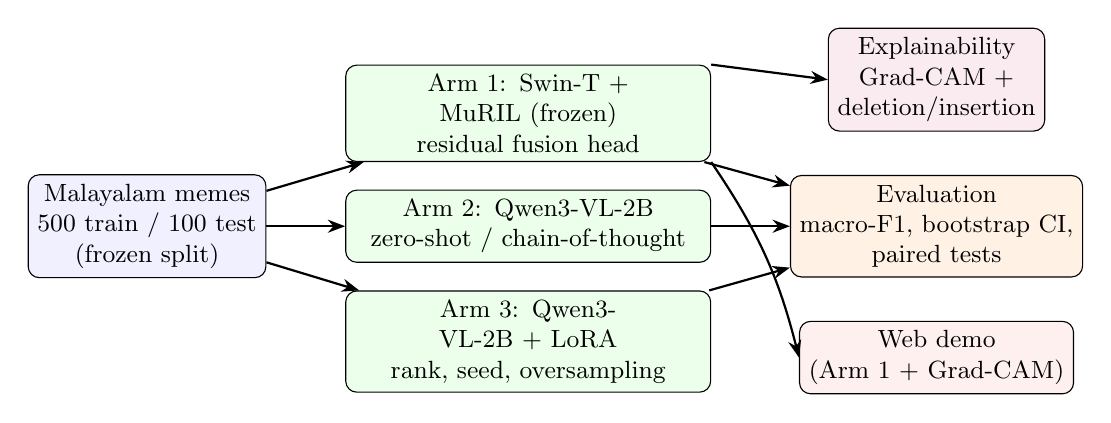
\begin{tikzpicture}[node distance=0.55cm and 0.7cm, every node/.style={font=\small},
  box/.style={draw, rounded corners, align=center, minimum height=0.9cm, minimum width=2.3cm, fill=blue!6},
  arm/.style={draw, rounded corners, align=center, minimum height=0.8cm, text width=4.4cm, fill=green!8},
  arr/.style={-{Stealth[length=2.2mm]}, thick}]
\node[box] (data) {Malayalam memes\\500 train / 100 test\\(frozen split)};
\node[arm, right=1.0cm of data] (a2) {Arm 2: Qwen3-VL-2B\\zero-shot / chain-of-thought};
\node[arm, above=0.35cm of a2] (a1) {Arm 1: Swin-T + MuRIL (frozen)\\residual fusion head};
\node[arm, below=0.35cm of a2] (a3) {Arm 3: Qwen3-VL-2B + LoRA\\rank, seed, oversampling};
\node[box, right=1.0cm of a2, fill=orange!10] (eval) {Evaluation\\macro-F1, bootstrap CI,\\paired tests};
\node[box, above=0.55cm of eval, fill=purple!8] (xai) {Explainability\\Grad-CAM +\\deletion/insertion};
\node[box, below=0.55cm of eval, fill=red!6] (demo) {Web demo\\(Arm 1 + Grad-CAM)};
\draw[arr] (data) -- (a1); \draw[arr] (data) -- (a2); \draw[arr] (data) -- (a3);
\draw[arr] (a1) -- (eval); \draw[arr] (a2) -- (eval); \draw[arr] (a3) -- (eval);
\draw[arr] (a1.north east) -- (xai.west);
\draw[arr] (a1.south east) to[bend left=10] (demo.west);
\end{tikzpicture}
\caption{As-built pipeline for Phase I.}
\label{fig:pipeline}
\end{figure}

\subsection{Dataset Selection}

The primary dataset is the Malayalam political-meme set of the DravidianLangTech 2026 shared task. Each meme has two labels: Level~1 (troll or support) and Level~2 (person, party or intersection; the source labels PERSON, PARTY, BOTH are normalised once, in the evaluation script). The training set has 500 images (477 troll, 23 support). The held-out test set has 100 images: 96 troll and 4 support at Level~1, and 54 person, 31 party and 15 intersection at Level~2. The test ids and labels were checked to be identical (100 of 100) across every arm's files. A 5-fold cross-validation split of the training set, stratified on Level~1 with seed 42, is used for Arm~1 model selection.

\subsection{Algorithm/Model Design}

\textbf{Arm 1: classical baseline.} A Swin-Tiny vision transformer \cite{liu2021swin} and MuRIL \cite{khanuja2021muril}, a BERT model pretrained on Indian languages, are both \emph{frozen}. Their 768-dimensional outputs are projected to 512 dimensions, concatenated and refined by two residual fusion blocks, $\mathbf{z}\leftarrow \mathrm{LN}(\mathbf{z}+\mathrm{MLP}(\mathbf{z}))$, then fed to two linear heads, one per label level. Only the projections, fusion blocks and heads are trained (AdamW, learning rate $10^{-3}$, batch size 16, 8 epochs), with class-weighted cross-entropy for imbalance. The text input is the text extracted from the meme image by Tesseract OCR \cite{smith2007tesseract}, because the source data contain no caption field.

\textbf{Arm 2: prompted VLM.} Qwen3-VL-2B-Instruct, quantised to 8 bits and run with MLX, is given the image only (no OCR text) and a task description asking for an INTENT (SUPPORT or CRITICISE) and a TARGET (PERSON, PARTY or BOTH). Two strategies are run with greedy decoding: \emph{zero-shot}, and \emph{chain-of-thought} \cite{wei2022cot} in which the model reasons for at most three short sentences and a second turn then asks only for the two answer lines \cite{kojima2022zeroshot}. The second turn is needed because the 2B model's free reasoning often repeats itself and exhausts the token budget before answering. Output that cannot be parsed counts as wrong. The prompt is label-neutral.

\textbf{Arm 3: LoRA fine-tuning.} The same Qwen3-VL-2B is adapted with LoRA \cite{hu2022lora} on the query and value projections of the language decoder only (vision tower frozen). The base configuration follows the SYNAPSE recipe: rank 4, $\alpha=8$, dropout 0.15, learning rate $5\times10^{-5}$, weight decay 0.1, effective batch size 8, 500 steps, and a structured INTENT/TARGET output. The ablation varies rank $\in\{4,8,16\}$ (with $\alpha=2\cdot$rank), seed $\in\{42,43,44\}$, and one oversampling condition in which ``party'' memes are duplicated twice and ``intersection'' memes four times in the training set only. The test set is never altered.

\subsection{Explainability and Faithfulness Method}

For Arm~1's image branch we compute Grad-CAM \cite{selvaraju2020gradcam} on the last-stage Swin feature map. Swin has no convolutional layer, so we use the $7\times7\times768$ output of its \texttt{forward\_features()} as the target. The backbone weights are frozen, so the input tensor itself is marked as requiring gradients, which lets gradients reach the feature map without any weight gradients being computed. Each cell of the map covers a $32\times32$ pixel patch of the $224\times224$ input.

To test faithfulness we use the deletion/insertion protocol of RISE \cite{petsiuk2018rise}. In \emph{deletion}, patches are removed in order of decreasing saliency and the model's probability for its predicted class is tracked; a faithful map makes this probability fall quickly, giving a low area under the curve (AUC). In \emph{insertion}, patches are revealed in the same order and a faithful map gives a high AUC. The control is the same procedure with a random patch order (5 seeds per image). We compare per image with a paired one-sided Wilcoxon signed-rank test. Only the image branch is perturbed; the OCR text is held fixed.

\subsection{Evaluation Protocol}

Every system is scored by one script. The metric is macro-F1 for each level, because accuracy would reward predicting the majority class (96\% of the test set is troll at Level~1). The average of the two levels, Avg-F1, is the shared-task ranking metric. Uncertainty is given by 95\% percentile bootstrap intervals (2000 resamples of the test set, seed 42). Differences from Arm~1 are tested with a paired bootstrap that reuses the same resamples for both systems. For Arm~3, configurations are judged by the mean and standard deviation over seeds, not by the best seed.

\subsection{Tools and Technologies}

Python 3.12, PyTorch, \texttt{timm} (Swin-Tiny), Hugging Face \texttt{transformers} (MuRIL), Tesseract OCR, MLX and \texttt{mlx-vlm} (Qwen3-VL-2B inference and LoRA training on Apple silicon), NumPy/pandas/scikit-learn for evaluation, FastAPI for the demonstration site, and Git for version control. All experiments ran on a 16\,GB Apple M-series laptop.

\subsection{Deviations from the Original Plan}
\label{sec:deviations}

The original plan assumed an A100 GPU, which was not available. Each affected item was replaced by the closest feasible experiment (Table~\ref{tab:deviations}); none was silently dropped.

\begin{table}[h]
\centering
\caption{Planned work and what was done instead.}
\label{tab:deviations}
\small
\begin{tabular}{p{4.0cm}p{5.4cm}p{5.6cm}}
\toprule
Planned & Done in Phase I & Reason \\
\midrule
Three 7B VLMs (Qwen2.5-VL-7B, LLaVA-1.6, PaliGemma) plus Gemini 2.5 Flash; zero/few-shot/CoT & Qwen3-VL-2B (8-bit); zero-shot and CoT; Gemini script written but not run & 7B in bf16 does not fit in 16\,GB; 2B is also the SYNAPSE backbone \\
QLoRA on three 7B models, 30--40 run grid & LoRA on Qwen3-VL-2B, 8 runs over rank, seed and oversampling & One run takes about 10 minutes locally \\
Explainability on VLM vision towers & Grad-CAM and faithfulness on Arm 1 only; shared record schema for later arms & Gradients through a 7B model need GPU memory \\
Hateful Memes and Tamil/Malayalam misogyny sets; cross-lingual transfer & Not run & Datasets were not obtained \\
LLM-generated synthetic augmentation & Deferred; class weighting (Arm 1) and oversampling (Arm 3) used instead & Schedule \\
\bottomrule
\end{tabular}
\end{table}

\subsection{Expected Outcomes}

We expected fine-tuning to beat prompting and prompting to beat a frozen-encoder classifier, and we expected the Grad-CAM maps to beat random ordering. Only the last of these is confirmed by the results (Chapter~4).

\subsection{Advantages of the Proposed Work}

The design isolates the effect of training by holding the backbone fixed, uses the same split and metric for every system, quantifies uncertainty instead of reporting single scores, and runs entirely on a laptop, so it can be reproduced without a GPU cluster.

\subsection{Limitations and Assumptions}

\begin{itemize}
    \item The test set has 100 images, of which only 4 are ``support'', so Level-1 macro-F1 rests on four examples.
    \item There is no validation split (500 train, 100 test). No configuration was tuned on held-out data, but a seed chosen after seeing test scores is a lead, not a result.
    \item A 2B model in 8 bits is not representative of 7B-scale VLMs; conclusions apply to this scale.
    \item Arm~1's OCR text has about 20\% empty extractions that were not manually verified.
    \item Faithfulness is measured with respect to the model, not to human judgement of plausibility.
\end{itemize}

\chapter{Experimentation and Result Analysis}
\label{chap.4}
This chapter reports how the three arms and the explainability method were evaluated. All numbers come from \texttt{outputs/evaluation/consolidated.md} and the per-arm result files in the project repository.

\section{Experimental Setup}

All experiments ran on a 16\,GB Apple M-series laptop with Python 3.12, PyTorch and \texttt{timm} for Arm~1, and MLX with \texttt{mlx-vlm} for Qwen3-VL-2B (8-bit) in Arms~2 and~3. No GPU server was used. Arm~1 was trained for 8 epochs; each Arm~3 run takes about 10 minutes.

\section{Datasets}

The Malayalam political-meme set of the DravidianLangTech 2026 shared task is used: 500 training and 100 held-out test images (Section~3.2.2). The Level-1 test distribution is 96 troll and 4 support; the Level-2 distribution is 54 person, 31 party and 15 intersection. Images were resized to 512\,px for the VLM arms and 224\,px for Swin-Tiny.

\section{Evaluation Metrics}

Macro-F1 at Level~1 and Level~2, and their mean (Avg-F1). Each score is given with a 95\% bootstrap interval. Per-class F1 and Level-2 confusion matrices are used for diagnosis. Faithfulness is measured with deletion and insertion AUC against a random-order control.

\section{Experimental Design}

\textbf{Baselines.} A majority-class predictor (always troll and person) shows what a model that learns nothing obtains. Arm~1 is the anchor against which all other systems are compared. Our own replication of the SYNAPSE recipe (Qwen3-VL-2B with LoRA, rank 4, 8-bit, MLX) is included as a reference, and the SYNAPSE paper's reported scores are shown separately and marked as not reproduced.

\subsection{Experimental Scenarios}

Arm~2: zero-shot and chain-of-thought. Arm~3: rank 4 (seeds 42, 43, 44), rank 4 with minority oversampling (seeds 42, 43, 44), rank 8 (seed 42) and rank 16 (seed 42).

\subsection{Parameter Tuning}

No hyperparameter search was performed. Arm~1 uses a single setting and Arm~3's base setting is taken from the SYNAPSE recipe. The only axes varied are LoRA rank, seed and oversampling, and the seeds were fixed in advance, not chosen on test scores.

\section{Results}

\subsection{Main comparison}

Table~\ref{tab:main} gives the main comparison. Arm~3 rows are the mean $\pm$ standard deviation over three seeds (sample standard deviation); rank 8 and 16 have one seed each.

\begin{table}[h]
\centering
\caption{Macro-F1 on the 100-image Malayalam test set. Brackets are 95\% bootstrap intervals for single runs; $\pm$ is the standard deviation over seeds.}
\label{tab:main}
\small
\begin{tabular}{p{6.2cm}ccc}
\toprule
System & Level-1 F1 & Level-2 F1 & Avg-F1 \\
\midrule
Majority class & 0.490 & 0.234 & 0.362 \\
Arm 1: Swin-Tiny + MuRIL & 0.508 [0.42, 0.61] & 0.394 [0.30, 0.49] & 0.451 [0.39, 0.51] \\
Arm 2: Qwen3-VL-2B zero-shot & 0.487 [0.47, 0.50] & \textbf{0.499} [0.38, 0.60] & 0.493 [0.44, 0.54] \\
Arm 2: Qwen3-VL-2B chain-of-thought & 0.482 [0.47, 0.50] & 0.429 [0.32, 0.53] & 0.455 [0.40, 0.51] \\
Arm 3: LoRA r4 (3 seeds) & 0.571 $\pm$ 0.059 & 0.349 $\pm$ 0.061 & 0.460 $\pm$ 0.055 \\
Arm 3: LoRA r4 + oversampling (3 seeds) & 0.557 $\pm$ 0.095 & 0.482 $\pm$ 0.026 & \textbf{0.520} $\pm$ 0.057 \\
Arm 3: LoRA r8 (1 seed) & 0.609 & 0.329 & 0.469 \\
Arm 3: LoRA r16 (1 seed) & 0.630 & 0.234 & 0.432 \\
SYNAPSE replication (ours) & 0.656 [0.48, 0.87] & 0.318 [0.24, 0.39] & 0.487 [0.38, 0.60] \\
\midrule
\emph{SYNAPSE paper (reported, not reproduced)} & 0.920 & 0.426 & 0.673 \\
\bottomrule
\end{tabular}
\end{table}

\subsection{Effect of random seed}

The same LoRA configuration gives very different results across seeds (Table~\ref{tab:seeds}). Rank-4 plain LoRA spans Avg-F1 0.38 to 0.51, and the oversampling configuration spans 0.47 to 0.60. The best single run (rank 4 with oversampling, seed 42: Level-1 0.692, Level-2 0.505, Avg 0.599) is therefore the most favourable of three seeds and should not be quoted on its own.

\begin{table}[h]
\centering
\caption{Arm 3 per-seed Avg-F1 (Level-1 / Level-2 in brackets).}
\label{tab:seeds}
\small
\begin{tabular}{lccc}
\toprule
Configuration & Seed 42 & Seed 43 & Seed 44 \\
\midrule
r4 & 0.510 (0.593 / 0.427) & 0.486 (0.630 / 0.343) & 0.384 (0.490 / 0.277) \\
r4 + oversampling & 0.599 (0.692 / 0.505) & 0.468 (0.490 / 0.445) & 0.493 (0.490 / 0.496) \\
\bottomrule
\end{tabular}
\end{table}

\subsection{Per-class behaviour}

Table~\ref{tab:perclass} shows why the Level-2 scores are low. Plain LoRA often predicts only the majority classes: rank 16 predicts ``person'' for every image, so its Level-2 F1 (0.234) equals the majority baseline exactly. The prompted model and the classical baseline recover about a third to 40\% of the intersection memes, and the best oversampled LoRA run recovers 11 of 15 (73\%), though other seeds of the same configuration recover only 1 to 4 of 15.

\begin{table}[h]
\centering
\caption{Per-class F1 (selected systems).}
\label{tab:perclass}
\small
\begin{tabular}{lccccc}
\toprule
System & troll & support & person & party & intersection \\
\midrule
Majority class & 0.980 & 0.000 & 0.701 & 0.000 & 0.000 \\
Arm 1 & 0.867 & 0.148 & 0.526 & 0.433 & 0.222 \\
Arm 2 zero-shot & 0.974 & 0.000 & 0.649 & 0.433 & 0.414 \\
Arm 3 r4 seed 42 & 0.963 & 0.222 & 0.726 & 0.222 & 0.333 \\
Arm 3 r4+os seed 42 & 0.985 & 0.400 & 0.733 & 0.270 & 0.512 \\
Arm 3 r16 seed 42 & 0.974 & 0.286 & 0.701 & 0.000 & 0.000 \\
\bottomrule
\end{tabular}
\end{table}

\subsection{Qualitative results: Grad-CAM}

Figure~\ref{fig:gradcam} shows Grad-CAM overlays for held-out memes, including a correct and an incorrect prediction. Single maps are illustrations only; the quantitative test in Section~\ref{sec:faith} supports any claim about them.

\begin{figure}[h]
\centering
\begin{subfigure}{0.31\textwidth}
\includegraphics[width=\textwidth]{35_level1_true-troll_pred-troll_correct.png}\caption{Level 1, correct (troll)}\end{subfigure}\hfill
\begin{subfigure}{0.31\textwidth}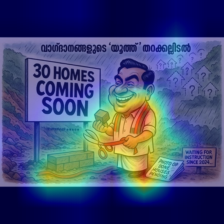
\includegraphics[width=\textwidth]{100_level1_true-troll_pred-support_wrong.png}\caption{Level 1, wrong (troll predicted support)}\end{subfigure}\hfill
\begin{subfigure}{0.31\textwidth}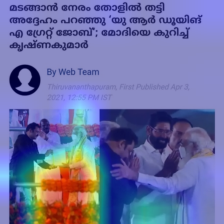
\includegraphics[width=\textwidth]{2_level2_true-person_pred-person_correct.png}\caption{Level 2, correct (person)}\end{subfigure}
\caption{Grad-CAM overlays on Arm 1's Swin-Tiny branch (test memes).}
\label{fig:gradcam}
\end{figure}

\subsection{Faithfulness of the heatmaps}
\label{sec:faith}

On all 100 test images, with five random orderings per image, Grad-CAM beats random patch order on both deletion and insertion at both levels (Table~\ref{tab:faith}). Grad-CAM is better on 82--93\% of images and the paired Wilcoxon test gives $p<10^{-11}$ in every case.

\begin{table}[h]
\centering
\caption{Deletion and insertion AUC, Arm 1, $n=100$ test images (mean).}
\label{tab:faith}
\small
\begin{tabular}{lcccc}
\toprule
Level & Del.\ CAM $\downarrow$ & Del.\ rand. & Ins.\ CAM $\uparrow$ & Ins.\ rand. \\
\midrule
1 (troll/support) & 0.588 & 0.791 & 0.864 & 0.736 \\
2 (person/party/inters.) & 0.354 & 0.551 & 0.627 & 0.511 \\
\bottomrule
\end{tabular}
\end{table}

\section{Analysis of Results}

\subsection{Observations}

\begin{enumerate}
    \item \textbf{Level~1 cannot separate the systems.} With four support memes, every Level-1 interval is wide (the upper end of one run reaches 1.00), and none of the Level-1 differences from Arm~1 is significant (paired bootstrap $p\ge0.44$).
    \item \textbf{At Level~2 the differences are small compared with the noise.} Zero-shot prompting (0.499) and oversampled LoRA (0.482 mean) exceed Arm~1 (0.394), but the paired bootstrap intervals on the difference include zero in every case ($p=0.11$ to $0.46$). The only significant differences at Level~2 are against the majority baseline and for the weakest LoRA runs, which are \emph{worse} than Arm~1 (rank 16, $p=0.003$; rank 4 seed 44, $p=0.029$).
    \item \textbf{Fine-tuning did not reliably beat prompting.} Plain LoRA (Avg 0.460) does not exceed zero-shot prompting of the same backbone (0.493) or the classical baseline (0.451), and often collapses to the majority class. Oversampling helps Level-2 across seeds (0.482 $\pm$ 0.026 versus 0.349 $\pm$ 0.061), but the Avg-F1 gain (0.520 versus 0.460) is about one standard deviation, so it is suggestive and not established with three seeds.
    \item \textbf{Chain-of-thought did not help.} It lowered Level-2 F1 from 0.499 to 0.429, consistent with the 2B model's tendency to produce degenerate reasoning.
    \item \textbf{Increasing LoRA rank did not help.} Rank 8 and 16 were no better than rank 4, though each has a single seed, so this is weak evidence.
    \item \textbf{The heatmaps are faithful but coarse.} The effect over random is large and consistent, so the maps reflect what the model uses at $7\times7$ resolution. They localise regions, not edges, and say nothing about the text branch.
\end{enumerate}

\subsection{Comparison with the published system}
\label{sec:paper-gap}

The SYNAPSE paper reports Level-1 0.920 and Level-2 0.426. Our direct replication of its recipe scored 0.656 and 0.318, and our best single run 0.692 and 0.505. We do not claim to match or beat the paper, for two reasons. First, a Level-1 score of 0.92 on our 100 images would require finding nearly all four support memes, whereas our replication found one of four at 96\% accuracy. Second, we have not confirmed that the paper's test split is the same as ours. Its figures come from our replication notes, not from the paper, and its class counts are not available to us. Treat the paper's numbers as \emph{reported, not reproduced and not shown to be comparable}. Our replication also differs from the paper in running at 8-bit on MLX rather than bf16 on a GPU.

\section{Comparative Analysis}

In summary, the Phase-I evidence supports four statements and no more:
(i) every learned system is above the majority baseline at Level~2 but not clearly above the classical baseline;
(ii) prompting a 2B VLM with no training is as good as, or better than, training it with LoRA on 500 images, unless minority oversampling is used;
(iii) seed variance is as large as the gap between methods, so single-run claims are unsafe; and
(iv) Grad-CAM on the classical baseline is demonstrably more faithful than chance.
The classical baseline is cheap, stable and explainable by gradient, and its intersection recall (33\%) is similar to the prompted model's (33--40\%). The VLM arms cost more to run and their gains over it are within noise.
 
\chapter{Conclusion and Scope for further Research}
\section{Conclusion}

We built and compared three approaches to two-level stance classification of Malayalam political memes on one frozen split and with one metric: a frozen-encoder classical baseline, a prompted Qwen3-VL-2B, and the same model fine-tuned with LoRA. The central result is that, on a 100-image test set with four ``support'' examples, no system is significantly better than the classical baseline, and the variation between random seeds of the same configuration is as large as the gaps between methods. Prompting without any training was competitive with LoRA fine-tuning on 500 images. Minority oversampling improved Level-2 results across three seeds, but the evidence for an overall gain is suggestive, not conclusive. Grad-CAM on the classical baseline is faithful, beating a random-order control on deletion and insertion for 82--93\% of 100 images ($p<10^{-11}$).

The study's main practical lesson is methodological: on small, imbalanced data, uncertainty must be reported, and one best seed is not a result. We also record, in full, where hardware limits forced deviations from the plan, and that the comparison with the published SYNAPSE scores remains unverified.

\section{Scope for Further Research (Phase II)}

\begin{enumerate}
    \item Run the 7B-scale VLMs and few-shot prompting on an A100, and Gemini~2.5~Flash through its API (script ready).
    \item Complete the oversampling study with more seeds and a validation split, so the gain can be tested rather than suggested.
    \item Build natural-language rationale generation and a cross-modal faithfulness score between rationale and heatmap, and extend Grad-CAM to the VLM vision tower and to the text branch.
    \item Obtain the Tamil and Malayalam misogyny set and the Hateful Memes reference set, and study checkpoint and prompt-language transfer separately.
    \item Obtain the SYNAPSE paper or contact its authors to confirm the test split and class counts, so a like-for-like comparison is possible.
    \item Evaluate LLM-generated augmentation of the minority classes against no augmentation and manual augmentation.
\end{enumerate}

\appendix
\chapter{title of appendix}
\section{Reproducibility and project structure}

All code is in the project repository, organised as \texttt{data/}, \texttt{arm1\_classical/}, \texttt{arm2\_vlm\_benchmark/}, \texttt{arm3\_peft\_finetune/}, \texttt{explainability/}, \texttt{evaluation/}, \texttt{demo/} and \texttt{website/}. Result files are in \texttt{outputs/}; \texttt{DEVIATIONS.md} lists every hardware-driven change. The single command \texttt{python -m evaluation.aggregate} regenerates all tables in Chapter~4.

\section{Notes on comparability with SYNAPSE}

See Section~\ref{sec:paper-gap}. Items we verified locally: the 100-image test ids and labels match across all arms; the test set has 96 troll and 4 support images; the training set has 477 troll and 23 support images. Items we did not verify: the paper's test-split size and class counts, and whether its 0.92 Level-1 score was obtained on this same split.


%\addcontentsline{toc}{chapter}{\textbf{References}}
\newpage
\renewcommand{\bibname}{References}
\bibliographystyle{ieeetr}
\addcontentsline{toc}{chapter}{References}
\bibliography{mybib}





\end{document}
	
	